\chapter{Licklider e Otlet}

\section{Licklider e le biblioteche del futuro}

Licklider (1915-1990) è stato uno psicoacustico che, nel 1950, iniziò ad appassionarsi
ai computer (al MIT). Partecipò sia alle "cene del Martedì" di Wiener\footnote{In cui si radunavano appassionati di cibernetica.} che 
alle Macy Conferences. Nel 1960 pubblicò un articolo intitolato \fancyglitter{Man-Computer Symbiosis} in cui
parla di una simbiosi uomo-computer in cui il computer è un collaboratore a cui si possono delegare
compiti di calcolo e di memorizzazione. 

\begin{figure}[h]
    \centering
    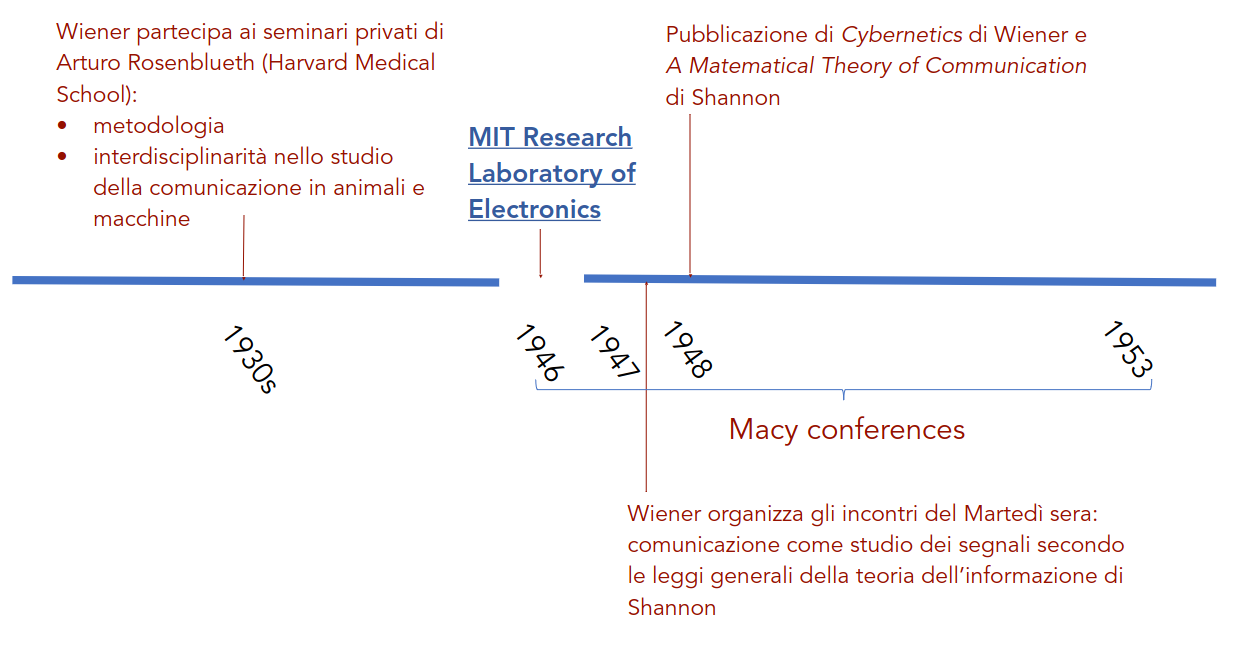
\includegraphics[scale=0.25]{images/MIT.png}
    \caption{Il MIT}
\end{figure}

\begin{itemize}
    \item [$\Rightarrow$] Licklider compie ricerche psico-acustiche (1943-1950);
    \item [$\Rightarrow$] Nel 1950 si appassiona ai computer;
    \item [$\Rightarrow$] Partecipa alle "cene del Martedì" di Wiener e alle Macy Conferences;
    \item [$\Rightarrow$] Lavora sul sistema SAGE (Semi-Automatic Ground Environment);
    \item [$\Rightarrow$] Vicepresidente della BBN (Bolt, Beranek and Newman), nel 1957 (inizia a lavorare sulle biblioteche del futuro);
    \item [$\Rightarrow$] Nel 1962 diventa direttore dell'ARPA (Advanced Research Projects Agency);
    \item [$\Rightarrow$] Convince Robert Fano a dirigere il progetto MAC (Multiple Access Computer)\footnote{Come visto nella prima parte del corso, nasce il \fancyglitter{time-sharing}.}.
\end{itemize}

\clm{}{}{C'è una leggenda secondo cui Licklider avrebbe persuaso Fano durante un viaggio in treno. Fano era un po'
scettico, ma conosceva Minsky, il ché era una garanzia di essere portati per l'informatica.
Inoltre aveva scritto un po' di programmi che funzionavano.}

\subsection{Man-Computer Symbiosis}

\paragraph{Prerequisiti per la simbiosi:}

\begin{itemize}
    \item [$\Rightarrow$] \fancyglitter{Time-sharing};
    \item [$\Rightarrow$] \fancyglitter{Estensione} della capacità e della velocità di accesso alla memoria;
    \item [$\Rightarrow$] \fancyglitter{Organizzazione} della memoria: accesso per nome o per schema con procedure di
    ricerca più veloci di quelle sequenziali (memorie associative, \fancyglitter{trie memory} di Fredkin);
    \item [$\Rightarrow$] \fancyglitter{Linguaggio}: gli ordini al computer specificano \fancyglitter{procedure}, all'uomo specificano \fancyglitter{obiettivi}.
\end{itemize}

\paragraph{Input e Output:}

\begin{itemize}
    \item [$\Rightarrow$] \fancyglitter{Riconoscimento} dei caratteri, \fancyglitter{immissione} dei dati in forma grafica;
    \item [$\Rightarrow$] \fancyglitter{Schermo gigante da parete} per la collaborazione e il coordinamento di gruppi\footnote{
        Vedrà la sua realizzazione negli anni '80 con il Computer-Supported Cooperative Work (CSCW), ma anche allo Xerox.
    };
    \item [$\Rightarrow$] \fancyglitter{Riconoscimento} del parlato.
\end{itemize}

\dfn{La rete intergalattica (1963)}{
    Nel 1963 Licklider scrive un articolo come Memorandum per i "Member and Affiliates of the Intergalactic Computer Network" 
    in cui invita le università a collegare i loro computer in una rete 
    per condividere risorse software.
}

\clm{}{}{Sulla West Coast, il movimento hippie\footnote{Nato nella zona di San Francisco.},
    concepisce l'idea di dare all'individuo la completa libertà che può essere messa
    in parallelo con l'idea di personal computer (non c'è condivisione di risorse, il computer è individuale).

}

\subsection{Le critiche al libro}

Nel libro \fancyglitter{Libraries of the Future} (1965) Licklider esplora
lo studio di classi di informazioni e domini di conoscenza, ci si concentra sui
concetti, sui principi e sulle idee dei libri più che sul loro aspetto tangibile.
Licklider vuole modificare gli \fancyglitter{schemi} impiegati per pensare alle biblioteche.

\begin{center}
    \fancyglitter{Componenti} $\rightarrow$ \fancyglitter{Pagine}

    \fancyglitter{Sottosistemi} $\rightarrow$ \fancyglitter{Volumi}

    \fancyglitter{Sistemi} $\rightarrow$ \fancyglitter{Biblioteche}
\end{center}

\begin{figure}[h]
    \centering
    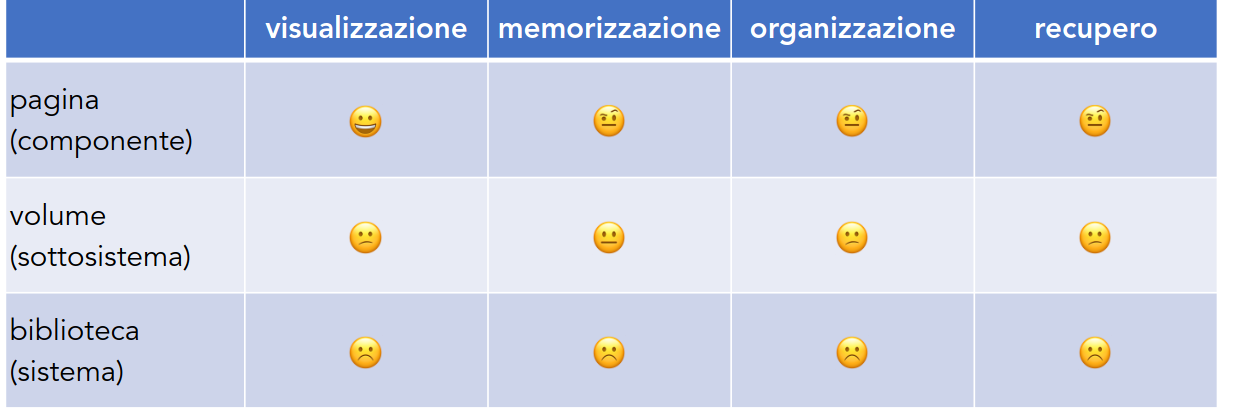
\includegraphics[scale=0.35]{images/Schemi.png}
    \caption{Schemi tradizionali.}
\end{figure}

\paragraph{Nelle prime pagine di Libraries of the Future vengono mosse delle critiche alla struttura e al concetto di libro:}

\begin{itemize}
    \item [$\Rightarrow$] La pagina può essere facilmente visualizzata e modificata, ma più pagine (libri) sono pesanti;
    \item [$\Rightarrow$] I libri contengono troppe informazioni e ciò nasconde le parti utili;
    \item [$\Rightarrow$] I libri sono scarsi anche dal punto della visualizzazione e del recupero delle informazioni\footnote{I problemi di indicizzazione già messi in evidenza da Bush.};
    \item [$\Rightarrow$] I testi sono passivi;
    \item [$\Rightarrow$] Dato che i libri (collezioni di pagine) diminuiscono i vantaggi della pagina, le biblioteche (collezioni di libri) diminuiscono i vantaggi dei libri.
\end{itemize}

\paragraph{Problema (passività della pagina stampata):}
\begin{itemize}
    \item [$\Rightarrow$] Il trasferimento di informazioni contenuta dai libri richiede lo spostamento del lettore, del libro o di entrambi;
    \item [$\Rightarrow$] Le operazioni di elaborazione del contenuto devono essere eseguite dal lettore.
    
\end{itemize}

\paragraph{Proposta di soluzione:} unire biblioteche e computer in un \fancyglitter{sistema procognitivo} (o biblioteca del futuro) per facilitare
l'interazione umana con informazione manipolabile e trasformabile.

\begin{figure}[h]
    \centering
    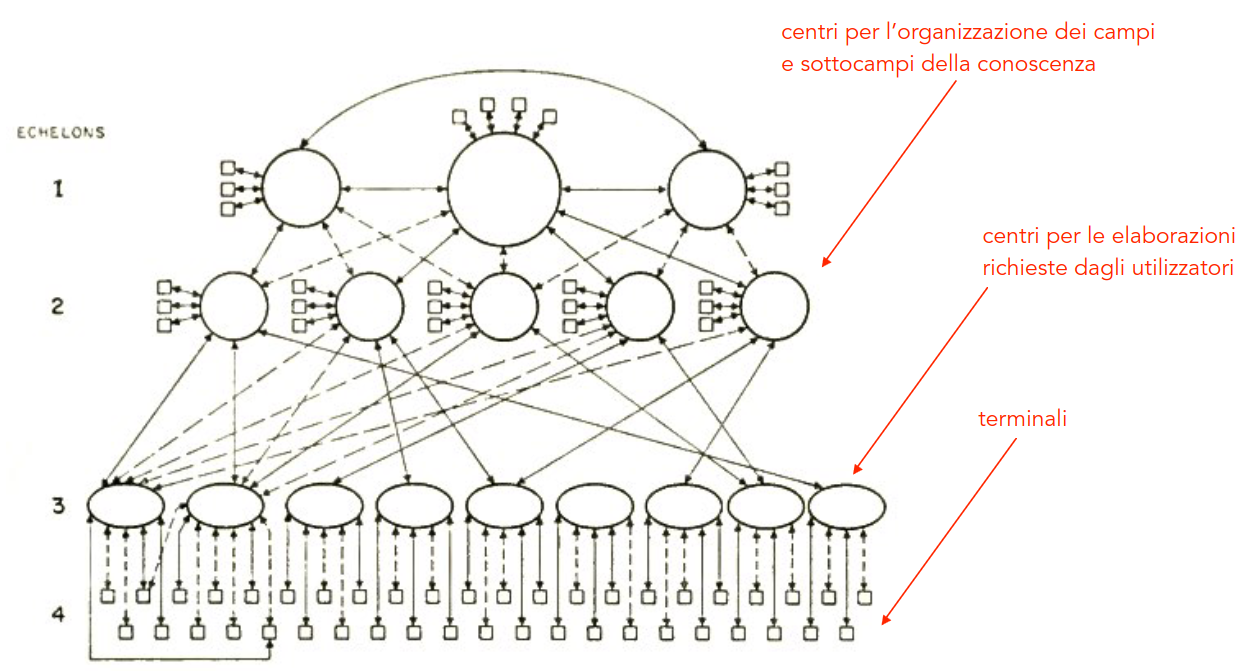
\includegraphics[scale=0.28]{images/SistemiP.png}
    \caption{Una biblioteca del futuro.}
\end{figure}

\paragraph{Riassunto dei difetti (\textcolor{red}{\XSolidBrush}) e dei pregi (\textcolor{green}{\Checkmark}) degli schemi tradizionali:}

\begin{itemize}
    \item [\textcolor{red}{\XSolidBrush}] Schema della biblioteca fisica con scaffali, schede, banchi di consegna, sale di lettura;
    \item [\textcolor{red}{\XSolidBrush}] Schema del libro fisico come archivio passivo di informazione stampata;
    \item [\textcolor{red}{\XSolidBrush}] Schema della pagina stampata come strumento per la memorizzazione a lungo termine;
    \item [\textcolor{green}{\Checkmark}] Gerarchie di segmenti di testo (carattere, parola, frase, paragrafo, capitolo, libro);
    \item [\textcolor{green}{\Checkmark}] La suddivisione in informazione testuale, grafica e figurativa;
    \item [\textcolor{green}{\Checkmark}] Le parti dei documenti (indice, prefazione, appendice, bibliografia, ecc.);
    \item [\textcolor{green}{\Checkmark}] Tipologie di pubblicazioni (libri, riviste, giornali, ecc.);
    \item [\textcolor{green}{\Checkmark}] Infrastrutture come catalogo, indice, etc..
\end{itemize}

\nt{Inoltre i "centri di calcolo" sono inefficaci nel tempo. Ed è proprio da
questo che si reinventa il calcolo in chiave contemporanea (time-sharing).}

\section{Otlet e la documentazione universale}

Paul Otlet (1868-1944) è stato un avvocato belga. Nel 1895 fonda l'Institut International de Bibliographie (IIB) a cui
si poteva scrivere per avere risposte in merito a domande bibliografiche. Nel 1904 Otlet e Henri La Fontaine, 
un avvocato e politico belga, crearono la \fancyglitter{Classificazione Decimale Universale} (una variante della Dewey). Nel 1919 Otlet creò il \fancyglitter{Palais Mondial}
e nel 1924 il \fancyglitter{Mundaneum}.

\subsection{Il futuro del libro}

Otlet affrontò il problema della \fancyglitter{crescita disordinata della letteratura}
nelle scienze sociali (1892 - Sulla bibliografia).
Per Otlet bisognava ridurre tutti i \fancyglitter{fatti osservati}, rimuovendo
tutte le \fancyglitter{interpretazioni possibili} trasformandoli in leggi, \fancyglitter{statistiche} e \fancyglitter{fonti}\footnote{Idea figlia del Positivismo.}.
Subito dopo gli elementi ottenuti verrebbero trasferiti su schede classificate con la 
Classificazione Decimale Universale. Così si arriverebbe alla creazione di un \fancyglitter{cervello artificiale}.
Nel 1918 Otlet pubblica "Trasformazioni nell'apparato bibliografico delle scienze" in cui viene messo in risalto il problema
della crescente produzione di libri\footnote{Ripreso da Bush.} e si parla di un miglioramento delle biblioteche\footnote{Ripreso da Licklider.}. In
questo testo vengono introdotte alcune idee:

\begin{itemize}
    \item [$\Rightarrow$] \fancyglitter{Repertorio};
    \item [$\Rightarrow$] \fancyglitter{Classificazione};
    \item [$\Rightarrow$] \fancyglitter{Ufficio della documentazione}.
\end{itemize}

\paragraph{Otlet criticò il libro:}

\begin{itemize}
    \item [$\Rightarrow$] Non è pratico per la consultazione di specifici passaggi;
    \item [$\Rightarrow$] È un'entità completa a cui non si può aggiungere nulla;
    \item [$\Rightarrow$] Rende difficile il collegamento di elementi correlati (richiede indicizzazione).
\end{itemize}

\nt{Probabilmente Licklider non conosceva Otlet, ma le conclusioni a cui sono giunti sono molto simili.}

\dfn{Repertorio}{
Il repertorio separa ciò che nel libro è unito e lo riduce a elementi
a cui viene dedicata una scheda. Non esiste la \newfancyglitter{rilegatura}, ma
le schede vengono tenute insieme in modo da poter essere riordinate, eliminate
o intercalate da nuove schede\footnote{Ricorda un quaderno ad anelli. Inoltre ci si può vedere un rimando all'idea di schede di Engelbart.}.
Il repertorio permette di \newfancyglitter{suddividere} un libro secondo il suo
contenuto: un libro è solo un'unica riga continua suddivisa per conformarsi alle pagine\footnote{un po' come se fosse scritto sul nastro di una macchina di Turing.}.
}

\clm{}{}{
    Il prof. Cardone esprime disappunto riguardo il significato di "pagina" di Otlet.
    La pagina ha una sua portata e persino i margini possono essere usati per esprimere qualcosa.
}

\dfn{Classificazione UDC}{
    La \newfancyglitter{Classificazione Decimale Universale} (UDC) è un sistema di classificazione bibliografica
    che si basa su un sistema di numeri decimali. È simile al linguggio ideale per 
    l'organizzazione della conoscenza. È decimale perché divisa in 10 classi, suddivise in almeno 10
    gruppi e ogni gruppo in almeno 10 divisioni.
}

\nt{La notazione UDC permette di creare senza limitazioni codici di classi.}

\dfn{Ufficio della documentazione}{
Le biblioteche sono \newfancyglitter{musei di libri}. Le loro collezioni sono 
relative alle esigenze di documentazione. Per rimediare a ciò, Otlet propose
l'idea di un \newfancyglitter{ufficio della documentazione} che avrebbe come punto
di partenza queste collezioni e dovrebbe stabilire dei collegamenti tra loro in modo da 
formare il \newfancyglitter{Libro Universale}\footnote{Questo ricorda ciò che saranno gli ipertesti di Nelson.}.
}

\subsection{Il Traité de documentation}

Nel 1934 Otlet pubblicò il \fancyglitter{Traité de documentation} in cui vengono sistematizzate
le proprie idee, parzialmente realizzate dal Mundaneum. Otlet studiò la possibilità di
\fancyglitter{macchine a supporto dei processi intellettuali}:

\begin{itemize}
    \item [$\Rightarrow$] Una \fancyglitter{scrivania} con superfici separate per la gestione di 
    progetti paralleli;
    \item [$\Rightarrow$] Macchine per la consultazione remota di documenti;
    \item [$\Rightarrow$] Una scrivania \fancyglitter{senza libri} ma con solo \fancyglitter{schermo e telefono}.
\end{itemize}

\nt{La standardizzazione della creazione, organizzazione, pubblicazione ed elaborazione
dei documenti favoriranno la creazione di una \fancyglitter{Rete Universale di Documentazione}.}

\clm{}{}{
    Nel 1968, Licklider collabora con Taylor (direttore di una sezione dello Xerox PARC) per un articolo,
    "The Computer as a Communication Device"\footnote{Scritto per via della sua esperienza nel laboratorio 
    di Engelbart.}, in cui si parla di una rete di computer che permetta la condivisione di risorse.
    Ossia il fatto che, nel giro di pochi anni, gli utenti comunicheranno più efficacemente
    attraverso una macchina che faccia a faccia. 

}
